\chapter{O Experimento}
\label{ch:07}

Neste capítulo falaremos sobre o modelo \textit{Encoder-Decoder} aplicado, bem como os hiperparâmetros utilizados. Além disso, será exibida a metodologia adotada para avaliação dos resultados e discussões sobre os resultados obtidos.

\section{Hiperparâmetros}
\label{sec:treinamento}

Os hiperparâmetros selecionados para a realização do experimento foram principalmente baseados em uma tarefa similar de \cite{cholletseq2seq}, em que textos são traduzidos de uma língua para outra utilizando o nível de caracter como referência.

Após alguns experimentos, o número de \textit{épocas} do modelo foi definido como 300. A escolha se deu após a verificação de que após esse valor o modelo tinha seu aprendizado estacionado.

Sem entrar em detalhes teóricos, também vale comentar os demais hiperparâmetros utilizados. As redes \textit{Encoder} e \textit{Decoder} são ambas arquiteturas do tipo LSTM com dimensão latente de 256 unidades cada (ou seja, apresentam uma camada intermediária com 256 nós). Para a otimização do modelo, foi utilizado o algoritmo \textit{Adam} (\cite{adam:2014}), disponível na API do \textit{Keras} (\cite{chollet2015keras}) com hiperparâmetros pré-definidos (taxa de aprendizado = 0.001, $\beta_{1}$=0.9, $\beta_{2}$=0.999, $\epsilon$ = Vazio, Decaimento = 0.0, amsgrad = Falso). A função de custo utilizada foi a de Entropia Cruzada Binária (\cite{francois2017deep}), já que temos que classificar uma série de valores como sendo \textbf{0}'s ou \textbf{1}'s. Além disso, o treinamento foi realizado em lotes (\textit{batches}) de 128 verbos com uma taxa de 20\% para validação cruzada. Por último, ainda baseado na tarefa de \cite{cholletseq2seq}, uma camada intermediária foi acrescentada entre o \textit{Decoder} e a camada de \textit{output}.

A Fig. \ref{fig:encoder-decoder} exibe a arquitetura completa do modelo.

\begin{figure}[H]
\center{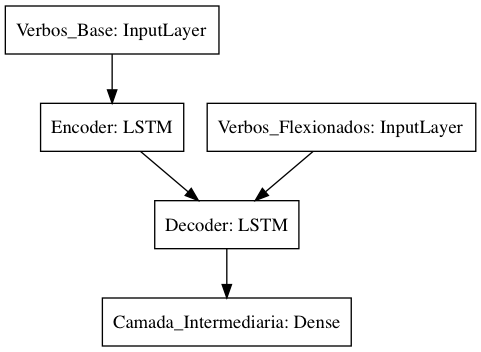
\includegraphics[width=0.6\textwidth]
{img/encoder-decoder.png}}
\caption{\label{fig:encoder-decoder} Arquitetura Final Utilizada.}
\end{figure}

\section{Metodologia para avaliação}
\label{sec:method}

 Para a avaliação dos resultados do modelo, foi utilizada uma técnica de validação cruzada chamada \textit{K-Fold} (\cite{kfold:2018}). A análise K-Fold permite que todos os verbos do corpus sejam testados. A técnica consiste, primeiramente, na formação de K subconjuntos de verbos mutuamente exclusivos de tamanhos próximos (idênticos caso a divisão por K seja exata). Em seguida, um desses subconjuntos é escolhido como o conjunto de teste enquanto que os K-1 restantes são utilizados como treino. O tamanho de K é definido a partir da escolha de proporção em que se deseja realizar a segmentação entre treino e teste, ou seja, para sempre manter a proporção de testes em 20\% de modo que estes verbos sejam sempre diferentes, o corpus precisa ser segmentado em 5 subconjuntos distintos. O desenho \ref{fig:kfold} ilustra o algoritmo. 

\definecolor{blue}{RGB}{159, 192, 176}
\definecolor{green}{RGB}{160, 227, 127}
\definecolor{orange}{RGB}{243, 188, 125}
\definecolor{red}{RGB}{253, 123, 84}
\definecolor{nephritis}{RGB}{39, 174, 96}
\definecolor{emerald}{RGB}{46, 204, 113}
\definecolor{turquoise}{RGB}{39, 174, 96}
\definecolor{green-sea}{RGB}{22, 160, 133}
\definecolor{purple}{RGB}{181, 124, 215}
% Tikzstyles for Computation Graphs

% nodes
\tikzstyle{noop} = [circle, draw=none, fill=red, minimum size = 10pt]
\tikzstyle{op} = [circle, draw=red, line width=1.5pt, fill=red!70, text=black, text centered, font=\bf \normalsize, minimum size = 25pt]

\tikzstyle{opintense} = [circle, draw=red, line width=1.5pt, fill=red!150, text=black, text centered, font=\bf \normalsize, minimum size = 25pt]


%new style
\tikzstyle{gp} = [circle, draw=red, line width=4pt, text=black, text centered, font=\bf \normalsize, minimum size = 4.cm]

\tikzstyle{box} = [rectangle, draw=red, line width=1.5pt, fill=red!70, text=black, align=center, font=\bf \normalsize, minimum size = 45pt]

\tikzstyle{box2} = [rectangle, draw=black, line width=0.9pt, text=black, align=center, font=\bf \normalsize, minimum size = 20pt]

\tikzstyle{box3} = [rectangle, draw=black, line width=0.9pt, fill=black, text=black, align=center, font=\bf \normalsize, minimum size = 20pt]

\tikzstyle{state} = [circle, draw=blue, line width=1.5pt, fill=blue!70, text=black, text centered, font=\bf \normalsize, minimum size = 25pt]

\tikzstyle{output} = [circle, draw=purple, line width=1.5pt, fill=purple!70, text=black, text centered, font=\bf \normalsize, minimum size = 25pt]


\tikzstyle{gradient} = [circle, draw=nephritis, line width=1.5pt, fill=nephritis!60, text=black, text centered, font=\bf \normalsize, minimum size = 25pt]
\tikzstyle{textonly} = [draw=none, fill=none, text centered, font=\bf \normalsize]
\tikzstyle{boxtextonly} = [draw=none, fill=none, align=center, font=\bf \normalsize]

\tikzstyle{normal} = [circle, draw=black, line width=1.0pt, fill=none, text=black, text centered, font=\bf \normalsize, minimum size = 20pt]


% edges
\tikzstyle{tedge}  = [draw, thick, >=latex, ->]
\tikzstyle{tedge_dashed}  = [draw, thick, >=latex, ->, dashed]
\tikzstyle{nedge}  = [draw, thick, >=latex]
\tikzstyle{nedge_dashed}  = [draw, thick, >=latex, dashed]


% namedscope
\tikzstyle{namedscope} = [circle, draw=orange, line width=1.5pt, fill=orange!60, align=center, inner sep=0pt]
\begin{figure}[ht!]
\centering

\scalebox{1.0}{
\begin{tikzpicture}[H]

%first
\node[box3] (box1) {};
\node[box2, right=0pt of box1] (box2) {};
\node[box2, right=0pt of box2] (box3) {};
\node[box2, right=0pt of box3] (box4) {};
\node[box2, right=0pt of box4] (box5);

%second
\node[box2, below=15pt of box1] (box6) {};
\node[box3, right=0pt of box6] (box7) {};
\node[box2, right=0pt of box7] (box8) {};
\node[box2, right=0pt of box8] (box9) {};
\node[box2, right=0pt of box9] (box10);

%third
\node[box2, below=15pt of box6] (box11) {};
\node[box2, right=0pt of box11] (box12) {};
\node[box3, right=0pt of box12] (box13) {};
\node[box2, right=0pt of box13] (box14) {};
\node[box2, right=0pt of box14] (box15);

%fourth
\node[box2, below=15pt of box11] (box16) {};
\node[box2, right=0pt of box16] (box17) {};
\node[box2, right=0pt of box17] (box18) {};
\node[box3, right=0pt of box18] (box19) {};
\node[box2, right=0pt of box19] (box20);

%fifth
\node[box2, below=15pt of box16] (box21) {};
\node[box2, right=0pt of box21] (box22) {};
\node[box2, right=0pt of box22] (box23) {};
\node[box2, right=0pt of box23] (box24) {};
\node[box3, right=0pt of box24] (box25);

%legenda
\node[box2, right=35pt of box10] (box26) {};
\node[textonly, right=5pt of box26] (box27) {Treino};
\node[box3, below=10pt of box26] (box28) {};
\node[textonly, right=5pt of box28] (box29) {Teste};



\end{tikzpicture}
}\caption{Técnica de segmentação do Corpus via K-Fold} 
\label{fig:kfold}
\end{figure}

Além disso, há ainda a vantagem do algoritmo de estratificação, ou seja, a certeza de que, em cada um dos treinamentos, as proporções das classes de verbos se mantenham no treinamento. Isso significa que, por exemplo, a classe de irregularidades do verbo “\textit{testar}” (testar $\rightarrow$ testo) que possui 20 verbos, terá sempre 16 verbos verbos no treinamento e 4 no teste. Assim, após os 5 treinamentos diferentes, todos os verbos da classe foram testados e fica garantido que havia verbos dessa classe no treinamento.

\subsection{Métrica de avaliação}

Para a avaliação dos resultados, considerou-se a métrica de \textit{Acurácia}. A acurácia pode ser obtida através da fórmula:

\begin{equation}
    Acurácia = \frac{contagem(acertos)}{contagem(total)}
\end{equation}

Ainda, define-se como um acerto um verbo predito exatamente igual ao esperado.

\section{Resultados}
\label{sec:resultado}
Como há um fator de aleatoriedade nas inicializações dos pesos, e também como os verbos de treino e teste são sorteados pelo algoritmo no momento da segmentação do K-Fold, os resultados da rede podem variar. Para a verificação dos resultados levando em consideração as variações, foram realizadas 30 análises K-Fold. Isso significa que cada verbo foi testado 30 vezes. Em média, temos que o modelo acerta 13.55\% dos verbos. Entretanto, a Fig. \ref{fig:acc} mostra um gráfico do tipo \textit{boxplot} (\cite{2004:bussab}) onde podemos verificar a variação da acurácia. Na figura, podemos notar que a taxa média de acerto do modelo desenvolvido se concentra entre 12.5-14.7\%, mas chega até 17\%.

\begin{figure}[H]
  \centering
  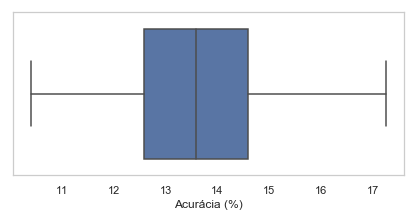
\includegraphics[width=0.6\linewidth]{img/mean_accuracy.png}
  \caption{Acurácia Para Todos os Verbos}
  \label{fig:acc}
\end{figure}

Ainda, agrupando todas as classes irregulares em apenas uma, é possível avaliar o desempenho do modelo comparativamente entre o grupo dos verbos regulares e o grupo de irregulares.
Nesse caso, a Fig. \ref{fig:boxplotsclasses} e a Tab. \ref{tab:acuraciamedia} mostra que o modelo obteve resultados melhores para a classe dos verbos regulares. 

\begin{figure}[H]
\begin{floatrow}
\ffigbox{%
  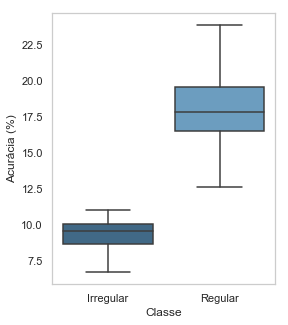
\includegraphics[width=0.8\linewidth]{img/boxplot_irregular_vs_regular.png}%
}{%
  \caption{Boxplots Para Acurácias por Classe}%
  \label{fig:boxplotsclasses}
}
\capbtabbox{%
\begin{tabular}{lll}
 & \textbf{Regulares} & \textbf{Irregulares} \\ \hline
\textbf{Acurácia Média} & 17.88 \% & 9.23 \% \\
\textbf{Acurácia DP} & 2.30 \% & 1.15 \% \\
\textbf{Acurácia Min}& 12.65 \% & 6.70 \%\\
\textbf{Acurácia Max}& 23.83 \% &  11.00 \%\\ \hline\\
& & \\ 
& & \\
& & \\
& & \\
\end{tabular}
}{%
  \caption{Acurácias Médias por Classe com Desvio Padrão (DP)}%
  \label{tab:acuraciamedia}
}
\end{floatrow}
\end{figure}




\subsection{Acurácia em cada classe}
\label{sec:prop}

Também é interessante avaliar o desempenho do modelo em cada uma das 16 classes formadas. Na Fig. \ref{fig:kfoldprop} observamos as acurácias de cada classe ordenadas pela proporção das mesmas no corpus. Nota-se que apesar da classe regular apresentar a maior proporção no corpus, as classes com maior acurácia são as classes dos verbos “botar” e “seguir”. Para avaliar a correlação entre a proporção no corpus e a acurácia foi utilizado o coeficiente de correlação de Pearson (\cite{2004:bussab}). Esse coeficiente assume valores entre -1 e 1, sendo que valores próximos às extremidades indicam maior correlação e valores próximos a zero indicam que as variáveis independem linearmente uma da outra. Para a interpretação do valor obtido utilizaremos a seguinte escala (\cite{pearson:1989}):

\begin{itemize}
    \item 0.9 para mais ou para menos indica uma correlação muito forte.
    \item0.7 a 0.9 positivo ou negativo indica uma correlação forte.
    \item0.5 a 0.7 positivo ou negativo indica uma correlação moderada.
    \item0.3 a 0.5 positivo ou negativo indica uma correlação fraca.
    \item0 a 0.3 positivo ou negativo indica uma correlação desprezível.
\end{itemize}

O coeficiente de correlação observado entre essas variáveis foi de \textbf{0.42}, o que indica uma correlação \textit{fraca}. 

\begin{figure}[H]
  \centering
  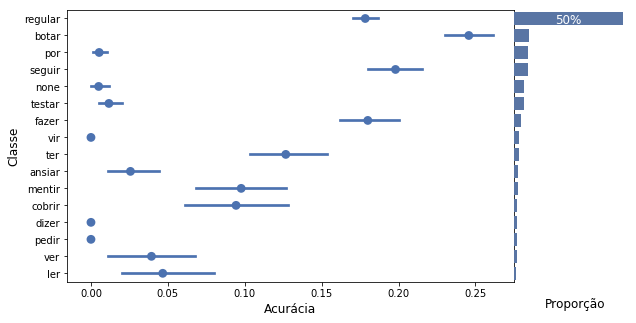
\includegraphics[width=0.8\linewidth]{img/proporxacc.png}
  \caption{Acurácia Para Cada Classe}
  \label{fig:kfoldprop}
\end{figure}

Para a análise dos resultados obtidos, utilizaremos o experimento K-Fold de acurácia total mais alta como referência (17\%, vide apêndice \ref{ap:results}). Como se pode observar, diferentes tipos de erros podem acontecer, sendo que alguns são piores do que outros. Vejamos, por exemplo, o verbo “parecer” (com transcrição fonética e RAD + VT = “parese”). Nesse caso vemos que o modelo produziu a forma “peresu”. Nota-se que essa transformação em que o modelo errou alguns traços de um único fone, é diferente do erro que ocorre com o verbo “retrair” (com transcrição fonética e RAD + VT = “hetrai”), para o qual o modelo produziu a forma “setEruu”. Vemos que no segundo caso, a forma produzida é praticamente incompreensível. %Desse modo, ao avaliarmos as diferentes classes de verbos, falaremos em \textit{erros incompreensíveis} para descrever os verbos cujas formas preditas apresentam erros de difícil interpretabilidade. 

Ao analisar os erros ocorridos na classe do verbo “Pôr” (Tab. \ref{tab:class_por}), verifica-se que 7/26 dos erros cometidos foram erros de \textit{regularização}, ou seja, o modelo se confundiu com a classe mais presente (a classe dos verbos regulares) e manteve o padrão de flexão regular.

\begin{table}[H]
\begin{tabular}{lll}
\multicolumn{1}{c}{Input} & \multicolumn{1}{c}{Output} & \multicolumn{1}{c}{Alvo} \\ \hline
kompo                     & kompu                      & kompoNu                  \\
despo                     & despu                      & despoNu                  \\
espo                      & espu                       & espoNu                   \\
antepo                    & antepu                     & antepoNu                 \\
supo                      & supu                       & supoNu                   \\
prosupo                   & prosupu                    & prosupoNu                \\
propo                     & propu                      & propoNu                  \\ \hline
\end{tabular}
\caption{Erros de regularização na classe do verbo “Pôr”}
\label{tab:class_por}
\end{table}

Em seguida, analisamos os verbos sem agrupamento (na Fig. \ref{fig:kfoldprop}, “none”). A acurácia baixa nesta classe era esperada pois não havia outros verbos no corpus para que o modelo conseguisse detectar possíveis padrões para fazer predições corretas. A Tab. \ref{tab:none} exibe alguns exemplos de erros nesta classe.

\begin{table}[H]
\begin{tabular}{lll}
\multicolumn{1}{c}{Input} & \multicolumn{1}{c}{Output} & \multicolumn{1}{c}{Alvo} \\ \hline
kabe                      & kabu                       & kaibu                    \\
idea                      & adeiu                      & ideiu                    \\
esta                      & estu                       & estou                    \\
traze                     & trasu                      & tragu                    \\
prove                     & provu                      & proveNu                  \\
estrea                    & estreiu                    & estrEiu                  \\ \hline
\end{tabular}
\caption{Exemplos de erros na classe sem agrupamento}
\label{tab:none}
\end{table}

Exemplos de erros na classe do verbo “testar” podem ser vistos na Tab. \ref{tab:class_testar}. Chama a atenção que, para o verbo “pegar”, o modelo acertou a flexão irregular transformando a vogal anterior meio-fechada em meio-aberta (e $\rightarrow$ \textepsilon), porém não acertou o traço de vozeamento para caracterizar o fone “g” ao invés de “k”, o que resultou na flexão equivocada de pegar $\rightarrow$ pEku.

\begin{table}[H]
\begin{tabular}{lll}
\multicolumn{1}{c}{Input} & \multicolumn{1}{c}{Output} & \multicolumn{1}{c}{Alvo} \\ \hline
seka                      & seku                       & sEku                     \\
leva                      & levu                       & lEvu                     \\
sega                      & segu                       & sEgu                     \\
fexa                      & fexu                       & fExu                     \\
pega                      & pEku                       & pEgu                     \\ \hline
\end{tabular}
\caption{Exemplos de erros na classe do verbo “testar”}
\label{tab:class_testar}
\end{table}

A classe do verbo “vir”, por sua vez, apresentou 5/11 de erros por regularização. Além disso, é interessante que para o verbo “revir” (\textit{hevi}) tenha flexionado como \textit{“heviju”}, flexão próxima ao grupo do verbo “ver”. A Tab. \ref{tab:class_vir} exibe alguns exemplos de erros nesta classe.

\begin{table}[H]
\begin{tabular}{lll}
\multicolumn{1}{c}{Input} & \multicolumn{1}{c}{Output} & \multicolumn{1}{c}{Alvo} \\ \hline
sobrevi                   & sobrevu                    & sobreveNu                \\
hevi                      & heviju                     & heveNu                   \\
adivi                     & adivu                      & adiveNu                  \\
avi                       & aviu                       & aveNu                    \\
provi                     & provu                      & proveNu                  \\ \hline
\end{tabular}
\caption{Exemplos de erros da classe “vir”}
\label{tab:class_vir}
\end{table}


\subsection{Acurácia e comprimento médio dos verbos nas classes}

Como o coeficiente de \textit{Pearson} observado entre a proporção das classes no corpus e a acurácia indicou uma correlação fraca, podemos buscar por outras variáveis que também possam influenciar no desempenho do modelo. Uma delas é o comprimento dos verbos. O verbo “3ntret3Nu” (entretenho), por exemplo, contém 9 fones para serem preditos. Como cada fone contém 20 traços, no total o modelo tem que conseguir prever 180 números. O verbo “falu” (falo), em contrapartida, possui 4 fones, ou seja, 80 números a serem preditos. Dessa forma, é natural pensar que quanto maior o número de predições necessárias, maior a probabilidade do modelo cometer algum erro. Com isso, a Figura \ref{fig:kfoldprop} exibe as acurácias das classes ordenadas de acordo com os comprimentos médios das mesmas. Na figura vemos que os grupos apresentam comprimentos médios que variam de 5 a 8 fones, mas com barras de confiança com limites próximos, indicando uma certa homogeneidade nesse aspecto.

No caso desse estudo, o coeficiente de \textit{Pearson} obtido foi de \textbf{0.39}, o que indica uma correlação também fraca entre estas variáveis. Entretanto, vemos nas barras de confiança que há pouca diferença significativa entre os comprimentos médios das classes. Além disso, é interessante notar que a classe em que o modelo apresentou melhor desempenho (a classe de “botar”) é simultaneamente uma classe com alta proporção no corpus e também apresenta o comprimento médio mais baixo do grupo.

\begin{figure}[H]
  \centering
  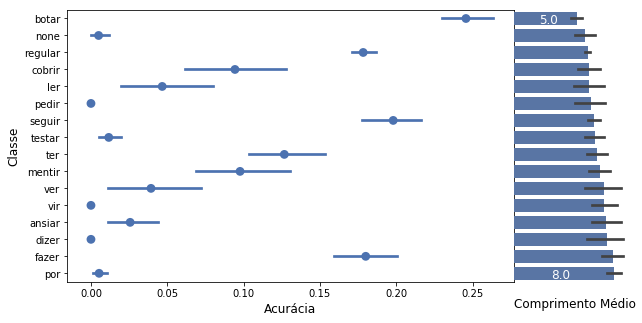
\includegraphics[width=0.8\linewidth]{img/comp_acc.png}
  \caption{Acurácia por Comprimento Médio}
  \label{fig:kfoldprop}
\end{figure}


% colocar no apendice os resultados
\section{Outros erros relevantes}
\label{sec:interesting}

Alguns erros interessantes como troca de classes e regularizações já foram apresentados na Seção \ref{sec:prop}, mas ainda há outros erros que merecem destaque. (Ver Apêndice \ref{ap:results} para tabela completa com Classe, Input, Output e Alvo)

Na classe de verbos sem agrupamento, um erro notável foi a flexão realizada para o verbo trazer (“trasu”), o que mostra que o modelo identificou o padrão de flexão da classe do verbo “fazer”. 

Na classe do verbo “pedir”, o modelo apresentou a flexão “espidu” para o verbo “expedir” (com alvo “espEsu” - “expeço”), o que denota uma possível confusão com a classe do verbo “conseguir”.

Nos verbos regulares nota-se a presença de vários erros devido a troca de apenas um traço fonético. Como por exemplo para o verbo “convidar”, o \textit{output} resultante foi “konviru” (trocou [\textbf{d}] - oclusiva, alveolar, sonora; por [\textbf{r}] - tepe, alveolar, sonora) . Para o verbo “convencer”, “konfensu” (trocou [\textbf{v}] - fricativa, lab. dental, sonora; por [\textbf{f}] - fricativa, lab. dental, surda).

Para os verbos da classe do verbo “seguir“, três verbos foram flexionados de acordo com a família do verbo “testar”. São eles: “ferir” (fEru), “vestir” (vEstu) e “repetir” (hepEtu).

A classe do verbo “ver” também apresentou erros interessantes: a confusão com a classe do verbo “vir” nos verbos “prever” (“preveNu”) e “entrever” (“entreveNu”). Também não acertou o alvo do verbo “rever” (hefexu), ficou faltando o traço de sonoridade nas duas últimas consoantes.

\section{Discussão}
\label{sec:discuss}

Durante a execução do presente trabalho, foi divulgado um estudo semelhante realizado pelos pesquisadores \cite{kirov:2018}. Nesse estudo, Kirov e Cotterell revisitam a questão dos verbos irregulares do inglês utilizando a arquitetura \textit{Encoder-Decoder}. Em razão da similaridade entre os estudos, é interessante pautar a discussão dos resultados obtidos através de uma comparação entre os mesmos. 

 No grupo dos verbos regulares, \cite{kirov:2018} obtiveram um desempenho próximo a 100\%. Entretanto, ao observarmos exclusivamente o desempenho no grupo dos verbos irregulares, a acurácia cai para 28.6\%. \cite{kirov:2018} explicam que os erros obtidos nessa circunstância foram erros de \textit{regularização}, e que em nenhum momento o modelo misturou regulares e irregulares como em “\textit{gaved}” (erro observado e criticado no modelo de \cite{rumelhart:1986}). Em números absolutos, os autores apresentaram um corpus composto por 4039 verbos (aproximadamente 10 vezes maior que o utilizado nesta pesquisa), sendo 168 destes considerados irregulares. Além disso, \cite{kirov:2018} realizaram uma partição aleatória tripla no corpus com proporções 80-10-10 para treino, desenvolvimento e teste. Desse modo, a base de teste dos pesquisadores continha apenas em torno de 17 verbos irregulares. Com uma acurácia de 28\%, isso significa que o modelo \textit{Encoder-Decoder} apresentado pelos autores acertou apenas cinco verbos irregulares. Sobre estes verbos, três deles eram verbos derivados de outros através de prefixação: \textit{retell} (derivado de \textit{tell}), \textit{partake} (derivado de \textit{take}) e \textit{withdraw} (derivado de \textit{draw}). Outro era o verbo \textit{sling}, similar a outros verbos presentes no treino (\textit{fling}, por exemplo). O último foi o verbo \textit{forsake}, cuja terminação se assemelha bastante ao verbo \textit{take}.

Além do modelo \textit{Encoder-Decoder} apresentado, \cite{kirov:2018} também reproduziram o modelo de regras de \cite{Albright2003RulesVA} (comentado na Seç. \ref{sec:compmot}) como referência (\textit{benchmark}) utilizando o mesmo corpus. Segundo os autores, para este modelo a acurácia dentre os verbos regulares ficou em torno de 95\%, porém não foi capaz de acertar nenhum verbo irregular em nenhuma das três partições realizadas. 

Em termos de pré-processamento, \cite{kirov:2018}
não explicitam a codificação utilizada, mas explicam que não utilizaram traços fonéticos como dados de entrada para a rede. A base de dados utilizada pelos autores foi a \textit{CELEX}, retirada de \cite{Baayen1993TheCL}, e era composta pelos verbos transcritos com a notação do AFI. 

Voltando ao modelo desenvolvido nesta pesquisa, observamos que a acurácia obtida no grupo dos verbos regulares foi a mais baixa em comparação aos demais trabalhos aqui referidos (com uma acurácia média igual a 13.55\% e máxima = 17\%). Entretanto, isto pode ser explicado em razão do tamanho do corpus necessário para o aprendizado em arquiteturas mais complexas, como é o caso do \textit{Encoder-Decoder}. Como visto, o modelo de \cite{kirov:2018} utilizou 4039 verbos para a tarefa (um corpus 10 vezes maior que o utilizado nesta pesquisa). Entretanto, como a ordem de grandeza obtida (423 verbos) estava próxima à ordem do conjunto de \cite{rumelhart:1986} (506 verbos), acreditava-se que o corpus obtido seria suficiente para a obtenção de acurácias mais altas. 

Com relação aos verbos irregulares, apesar da acurácia média obtida ter sido 9.23\%, em números absolutos isso representa em torno de 20 verbos. Dessa forma, é difícil comparar os dois modelos nessa questão. Se por um lado o montante de verbos regulares obtidos por \cite{kirov:2018} os levou a quase 100\% de acurácia nesse grupo, também foi um fator desfavorável para o desempenhoo no grupo dos verbos irregulares. Também pode-se questionar se os cinco verbos corretos obtidos por \cite{kirov:2018} refletem de fato o potencial de 23\% de acurácia do modelo. Certamente a discussão seria mais interessante caso tivéssemos uma acurácia média com desvioc-padrões, como foi apresentado neste trabalho. Em comparação com os resultados do \textit{benchmark} de \cite{kirov:2018} (baseado no modelo de \cite{Albright2003RulesVA}), o modelo apresentado nesta pesquisa apresentou desempenho melhor nesse quesito (9.23\% contra 0\%). 

No que diz respeito aos tipos de erros encontrados, pode-se dizer que alguns erros observados nesta pesquisa mostram-se bastante incompreensíveis de um ponto de vista linguístico em comparação aos apresentados por \cite{kirov:2018} (erros como “\textit{aAsaxu}”, como \textit{output} para o verbo “\textit{analisar}”). Entretanto, como os processos de codificação e decodificação, bem como os tamanhos dos \textit{corpus} e os objetos dos estudos são diferentes (traços fonéticos x fonemas), também seria injusta uma comparação entre os modelos nesse sentido.

Sobre o fato das métricas das correlações obtidas entre acurácia e tamanho médio e proporção no corpus não terem se mostrado fortes,
 chama a atenção que a classe do verbo “botar”. Essa classe, além ter apresentado a maior acurácia, apresenta também proporção no corpus  alta e é também a classe com comprimento médio mais baixo. Desse modo, supõe-se que estes fatores combinados tenham levado a esse resultado. Uma análise multivariada poderia ser feita para investigar a suposição em mais profundidade.

Para concluir a discussão, pode-se dizer que o desempenho do modelo \textit{Encoder-Decoder} está bastante condicionado à quantidade do corpus disponível. De certo que para qualquer modelo de Rede Neural, quanto maior o número de exemplos, melhor. Entretanto, vemos também que quanto mais profunda a arquitetura do modelo de Rede Neural, maior a demanda por mais exemplos. Ainda, vimos que a questão da proporção da classe de verbos irregulares mostrou-se relevante. Desse modo, os resultados obtidos nesta pesquisa não permitem dizer que o modelo \textit{Encoder-Decoder} seja adequado para esta tarefa. Contudo, pode-se argumentar que, como os processos de codificação e decodificação são módulos independentes da arquitetura, essa conclusão a respeito do modelo \textit{Encoder-Decoder} seria injusta. E que para que pudéssemos chegar a conclusões mais contundentes, mais experimentos deveriam ser realizados. Dito isto, direções para possíveis trabalhos futuros serão abordadas no próximo capítulo (Cap. \ref{ch:08}). 

  